\section{Ergebnisse}

\subsection{Vorhersage der Daten\"ubertragungsraten}

\subsubsection{Extreme Gradient Boosting}

Die Out-of-Sample Vorhersagen der Da\-ten\"uber\-tra\-gungs\-ra\-ten des Extreme Gradient Boosting Modells
finden sich in Abbildung~\ref{fig:datarate-predictions-xgboost}.
Man erkennt, dass sich die Verteilungen der Datenraten mitunter stark je nach Szenario und Anbieter unterscheiden.
Vor allem f\"allt auf, dass der Anbieter Vodafone eine wesentlich h\"ohere Variation in den Download-Raten vorweist,
alls die \"ubrigen Anbieter.
Insgesamt lassen sich anhand dieser Vorhersagen allerdings keine systematischen Unregelm\"a{\ss}igkeiten erkennen.
\begin{figure}
\centering
\begin{subfigure}{\textwidth}
    \centering
    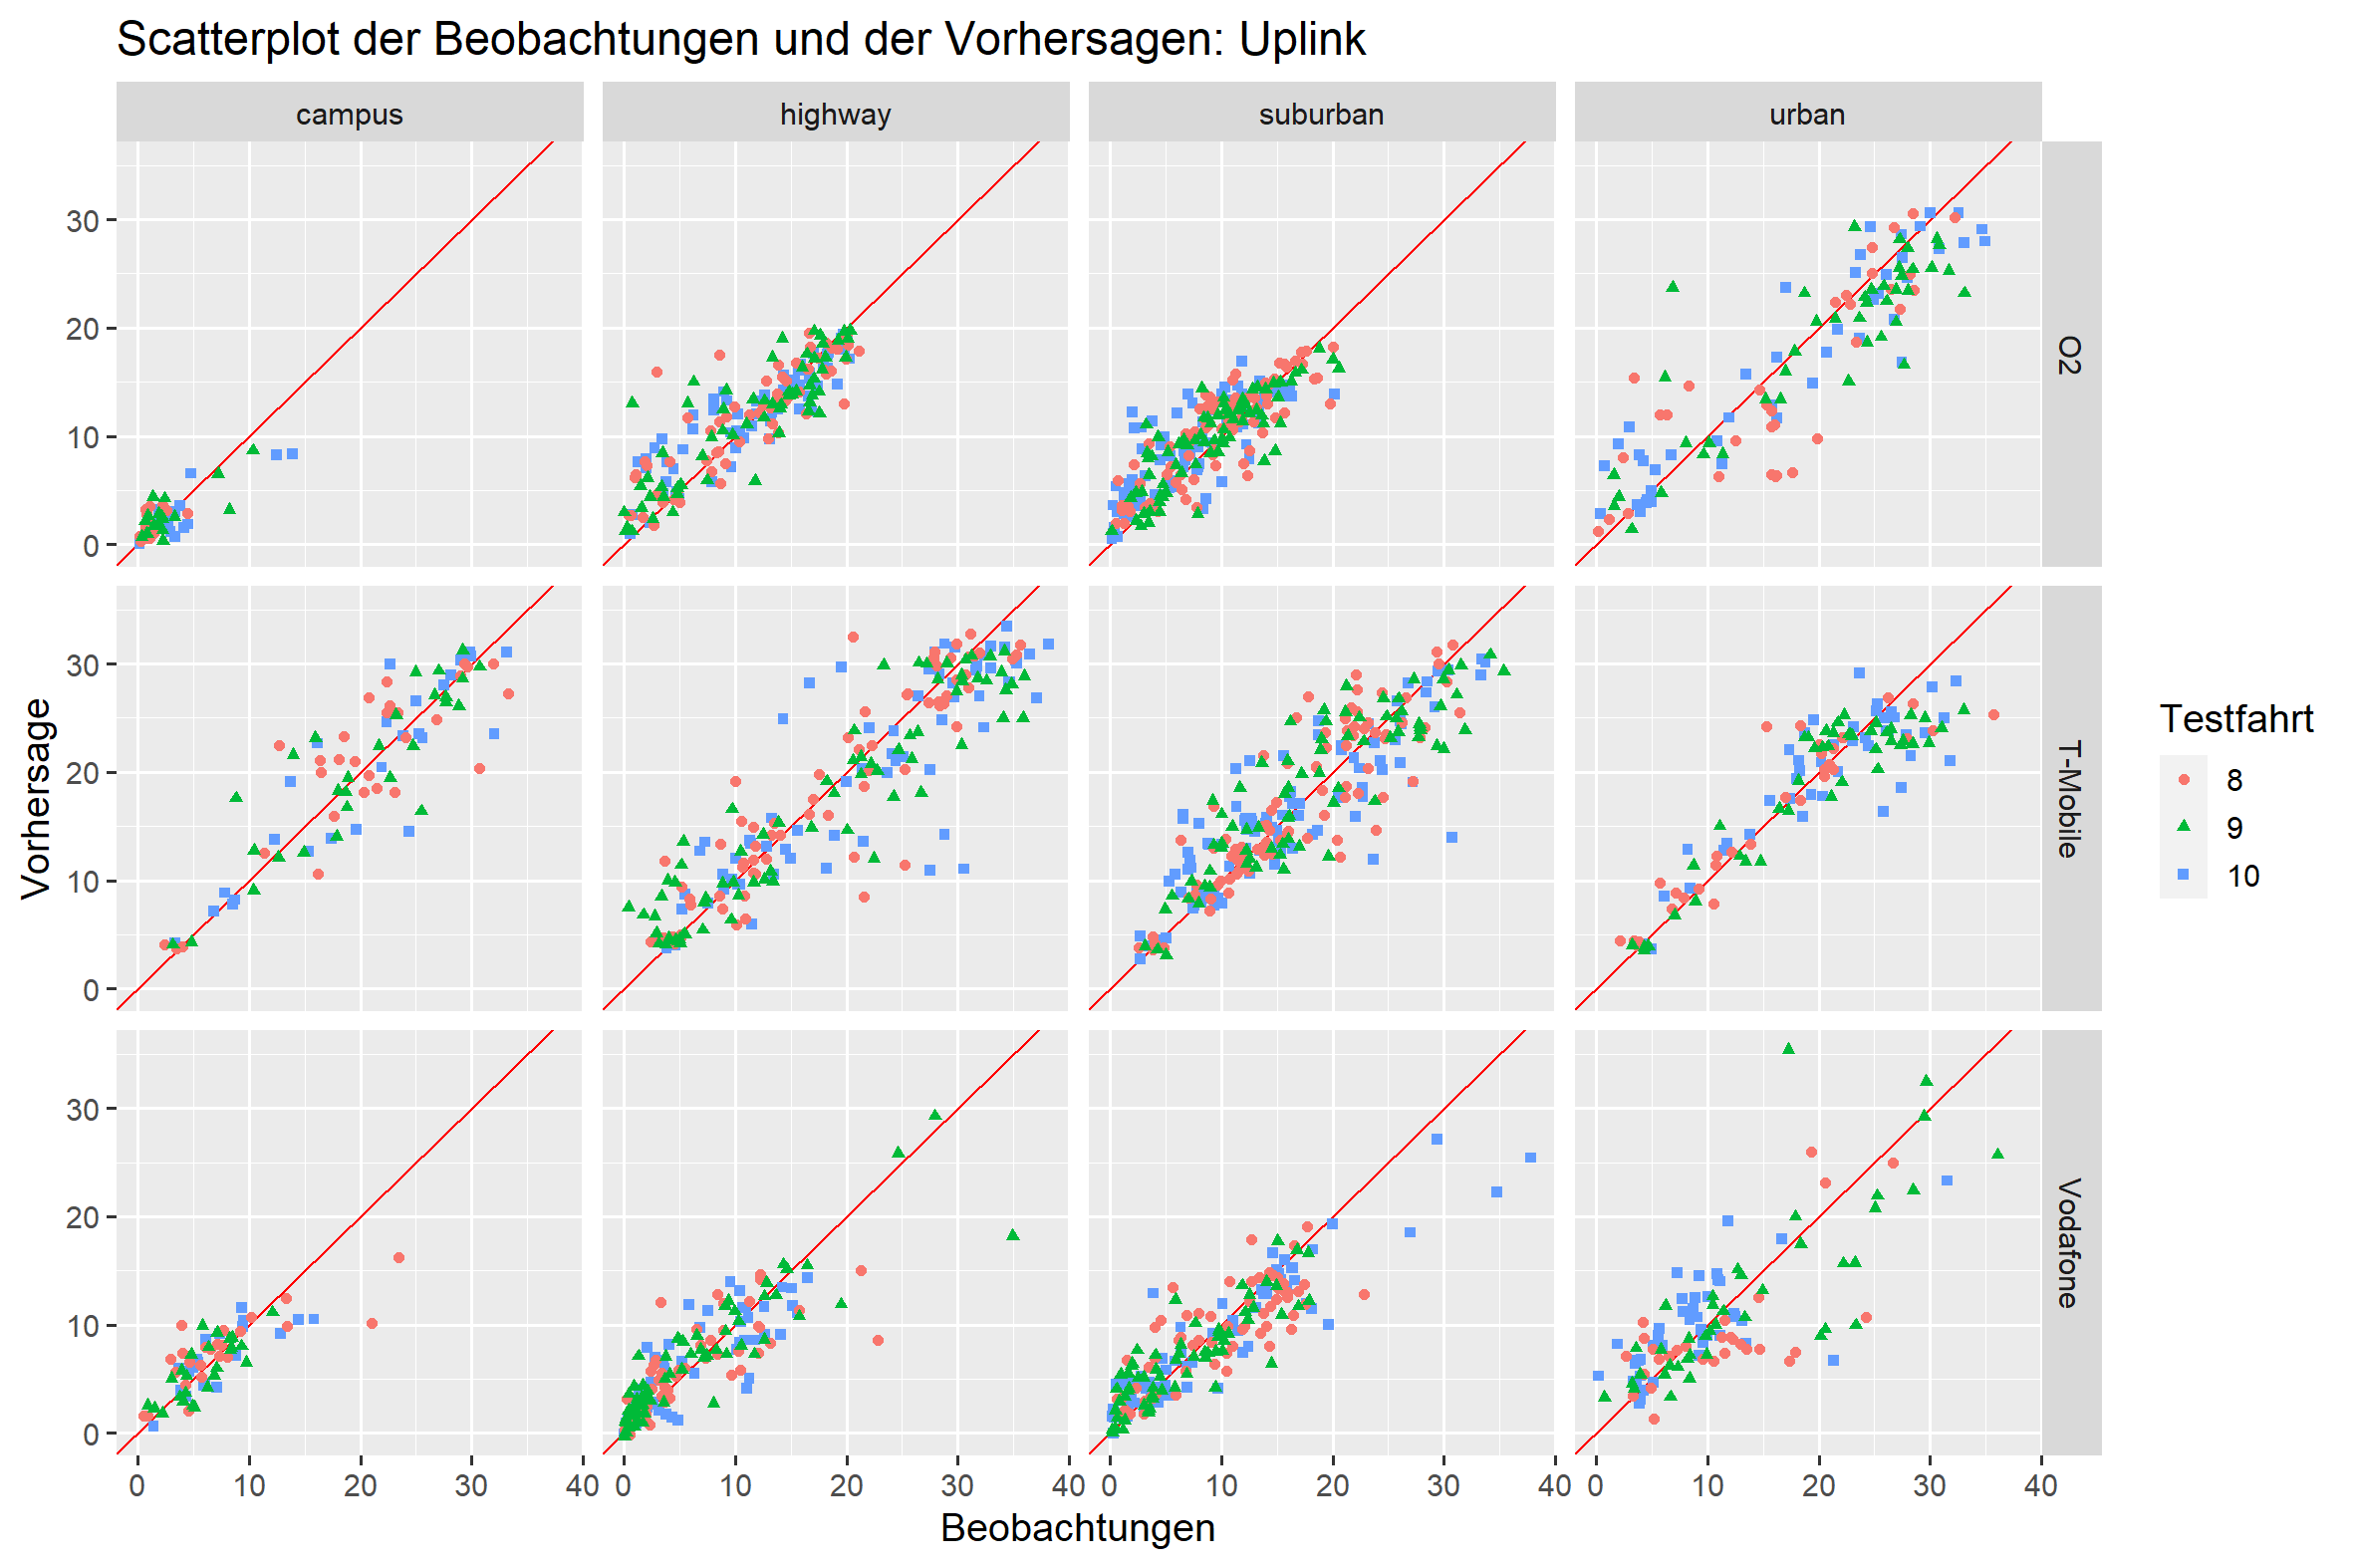
\includegraphics[width=\textwidth]{abbildungen/xgboost_predictions_ul}
\end{subfigure}
\begin{subfigure}{\textwidth}
    \centering
    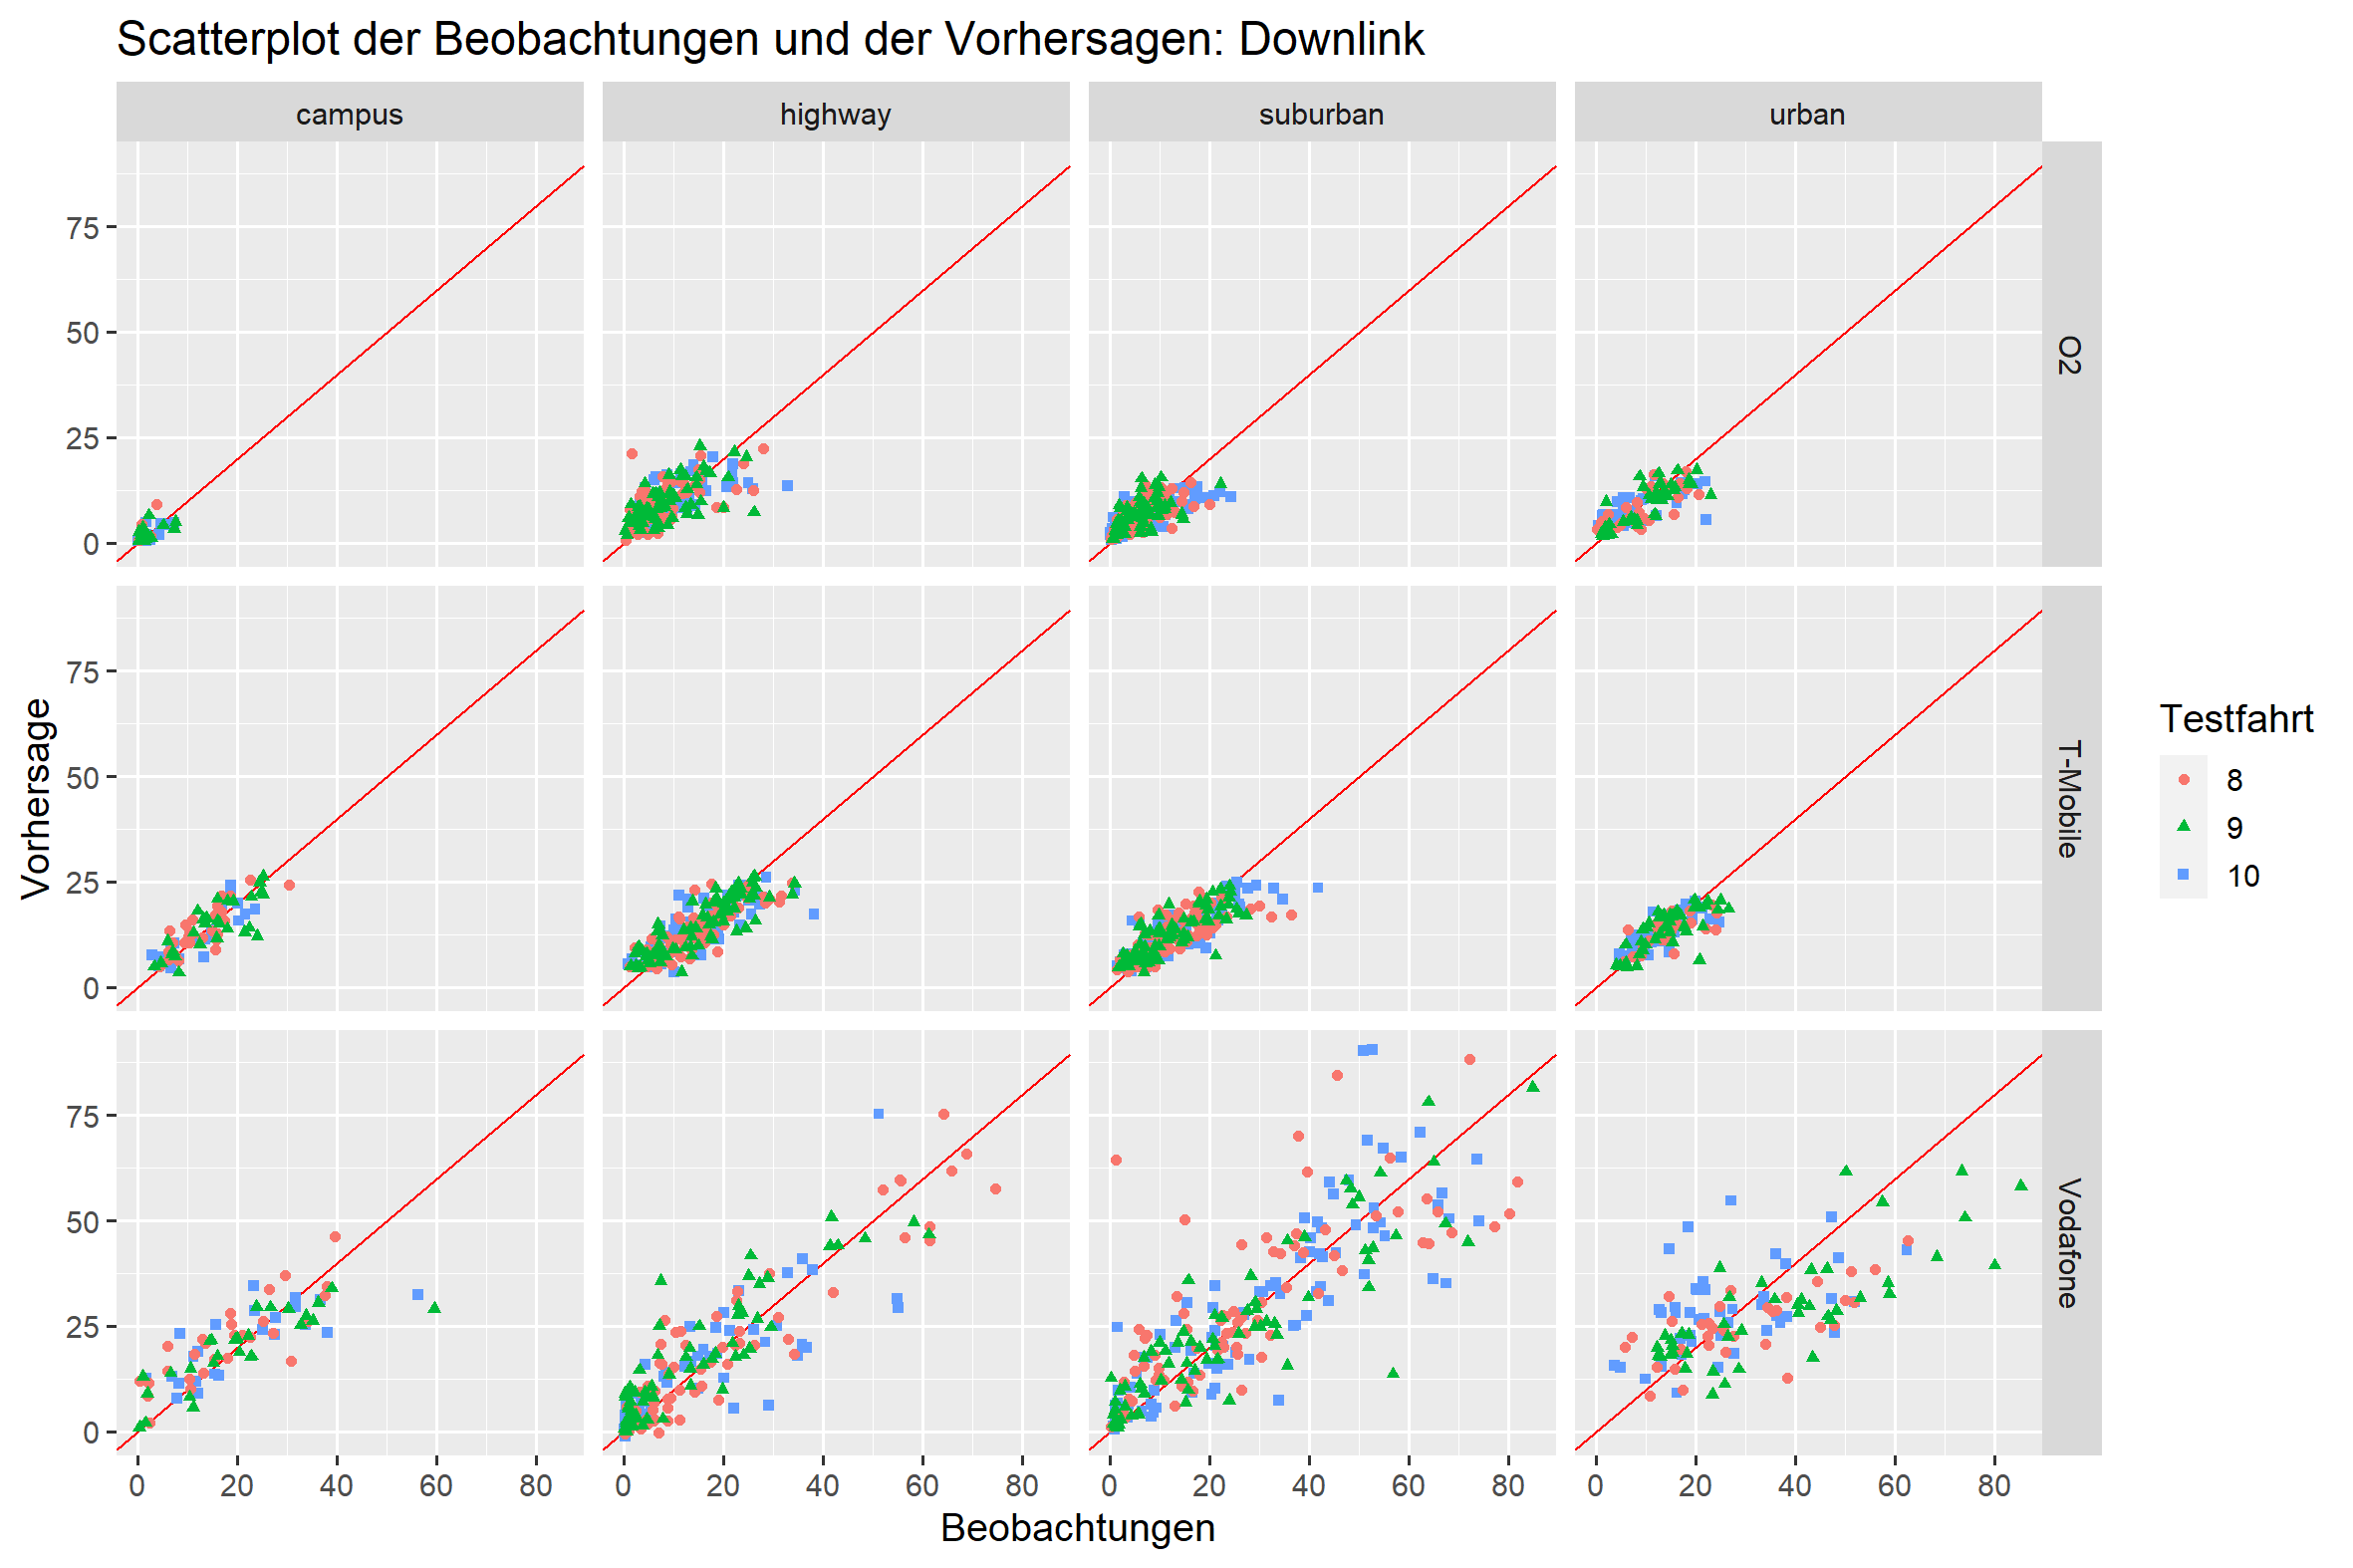
\includegraphics[width=\textwidth]{abbildungen/xgboost_predictions_dl}
\end{subfigure}
\caption{Out-of-Sample Vorhersagen der Datenraten f\"ur Extreme Gradient Boosting.}
\label{fig:datarate-predictions-xgboost}
\end{figure}

\subsubsection{Regression mit ARMA-Fehlern}

F\"ur die lineare Regression mit ARMA-Fehlern finden sich die Out-of-Sample Vorhersagen in Abbildung~\ref{fig:datarate-predictions-arma}.
Vergleicht man diese mit den Vorhersagen des Extreme Gradient Boosting, so fallen hier schon etwas st\"arkere systematische
Abweichungen ins Auge.
Beispielsweise scheint es so, dass im \textit{urban} Szenario f\"ur den Anbieter O2 h\"ohere Upload-Raten systematisch untersch\"atzt
und niedrigere Upload-Raten systematisch \"ubersch\"atzt werden.
Dies gibt einen ersten Aufschluss dar\"uber, dass das Modell m\"oglicherweise nicht expressiv genug sein k\"onnte,
um die Zusammenh\"ange in den Daten zu erfassen.
\begin{figure}
\centering
\begin{subfigure}{\textwidth}
    \centering
    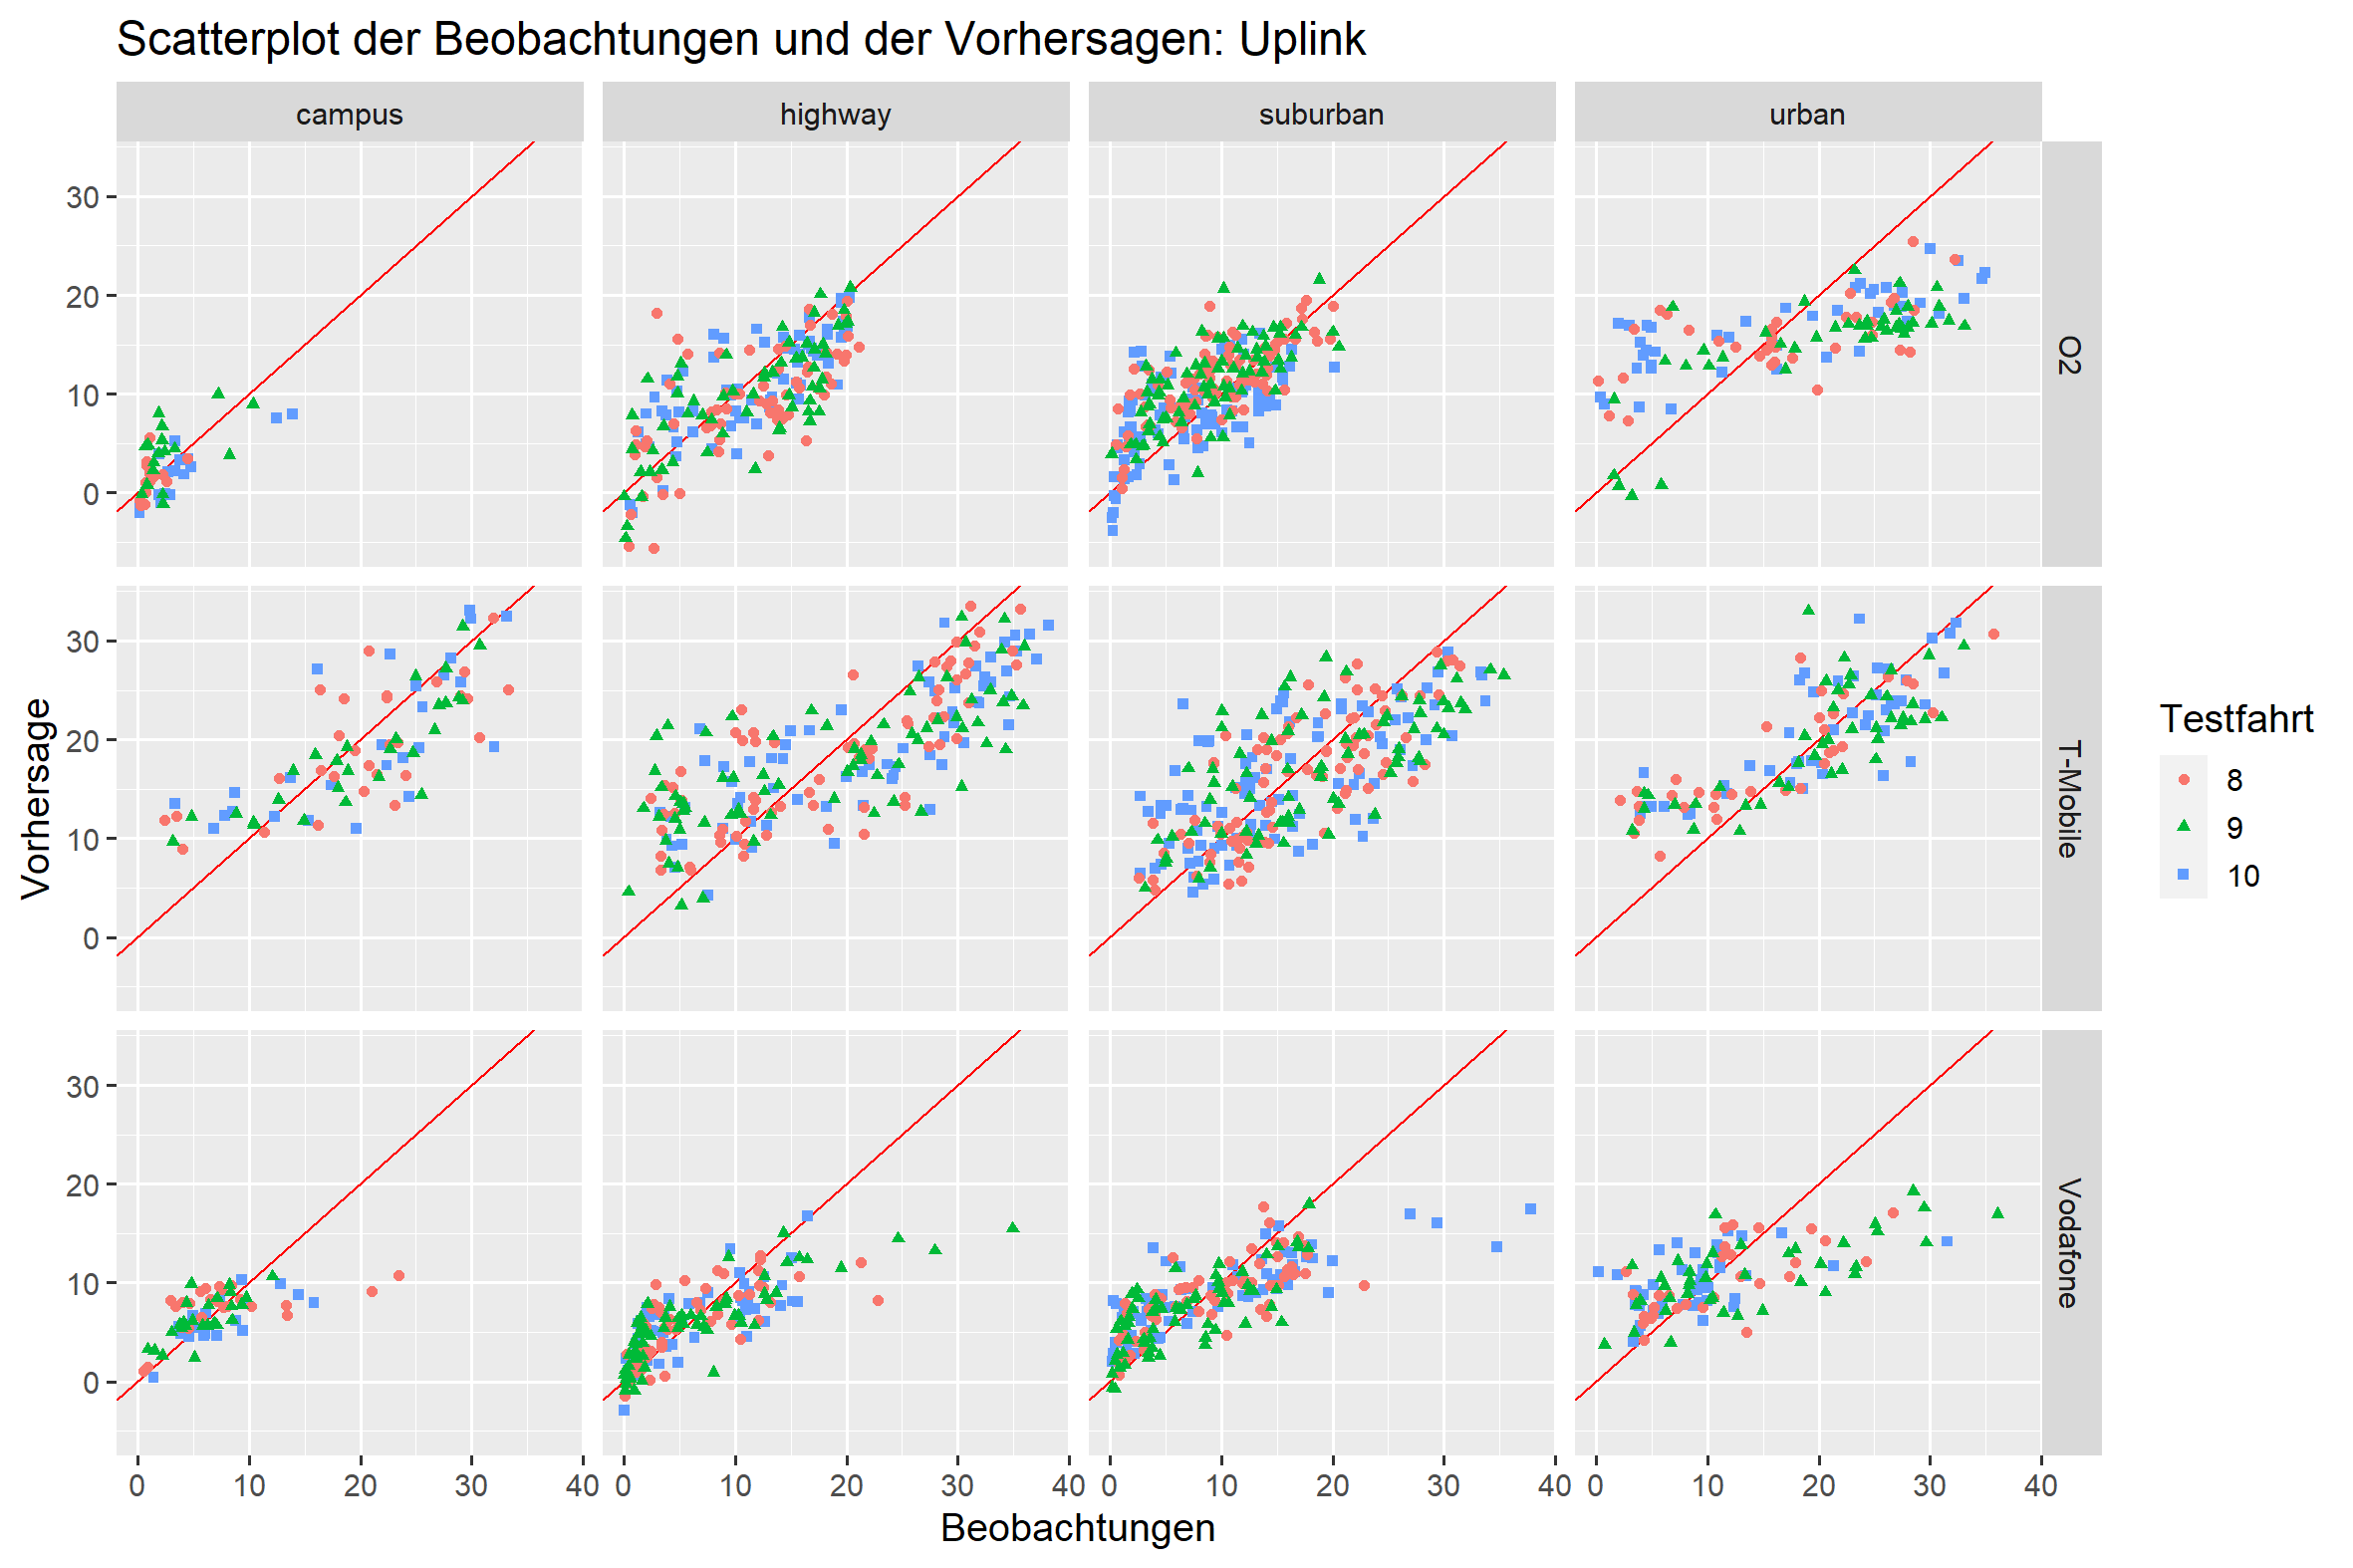
\includegraphics[width=\textwidth]{abbildungen/arma_predictions_ul}
\end{subfigure}
\begin{subfigure}{\textwidth}
    \centering
    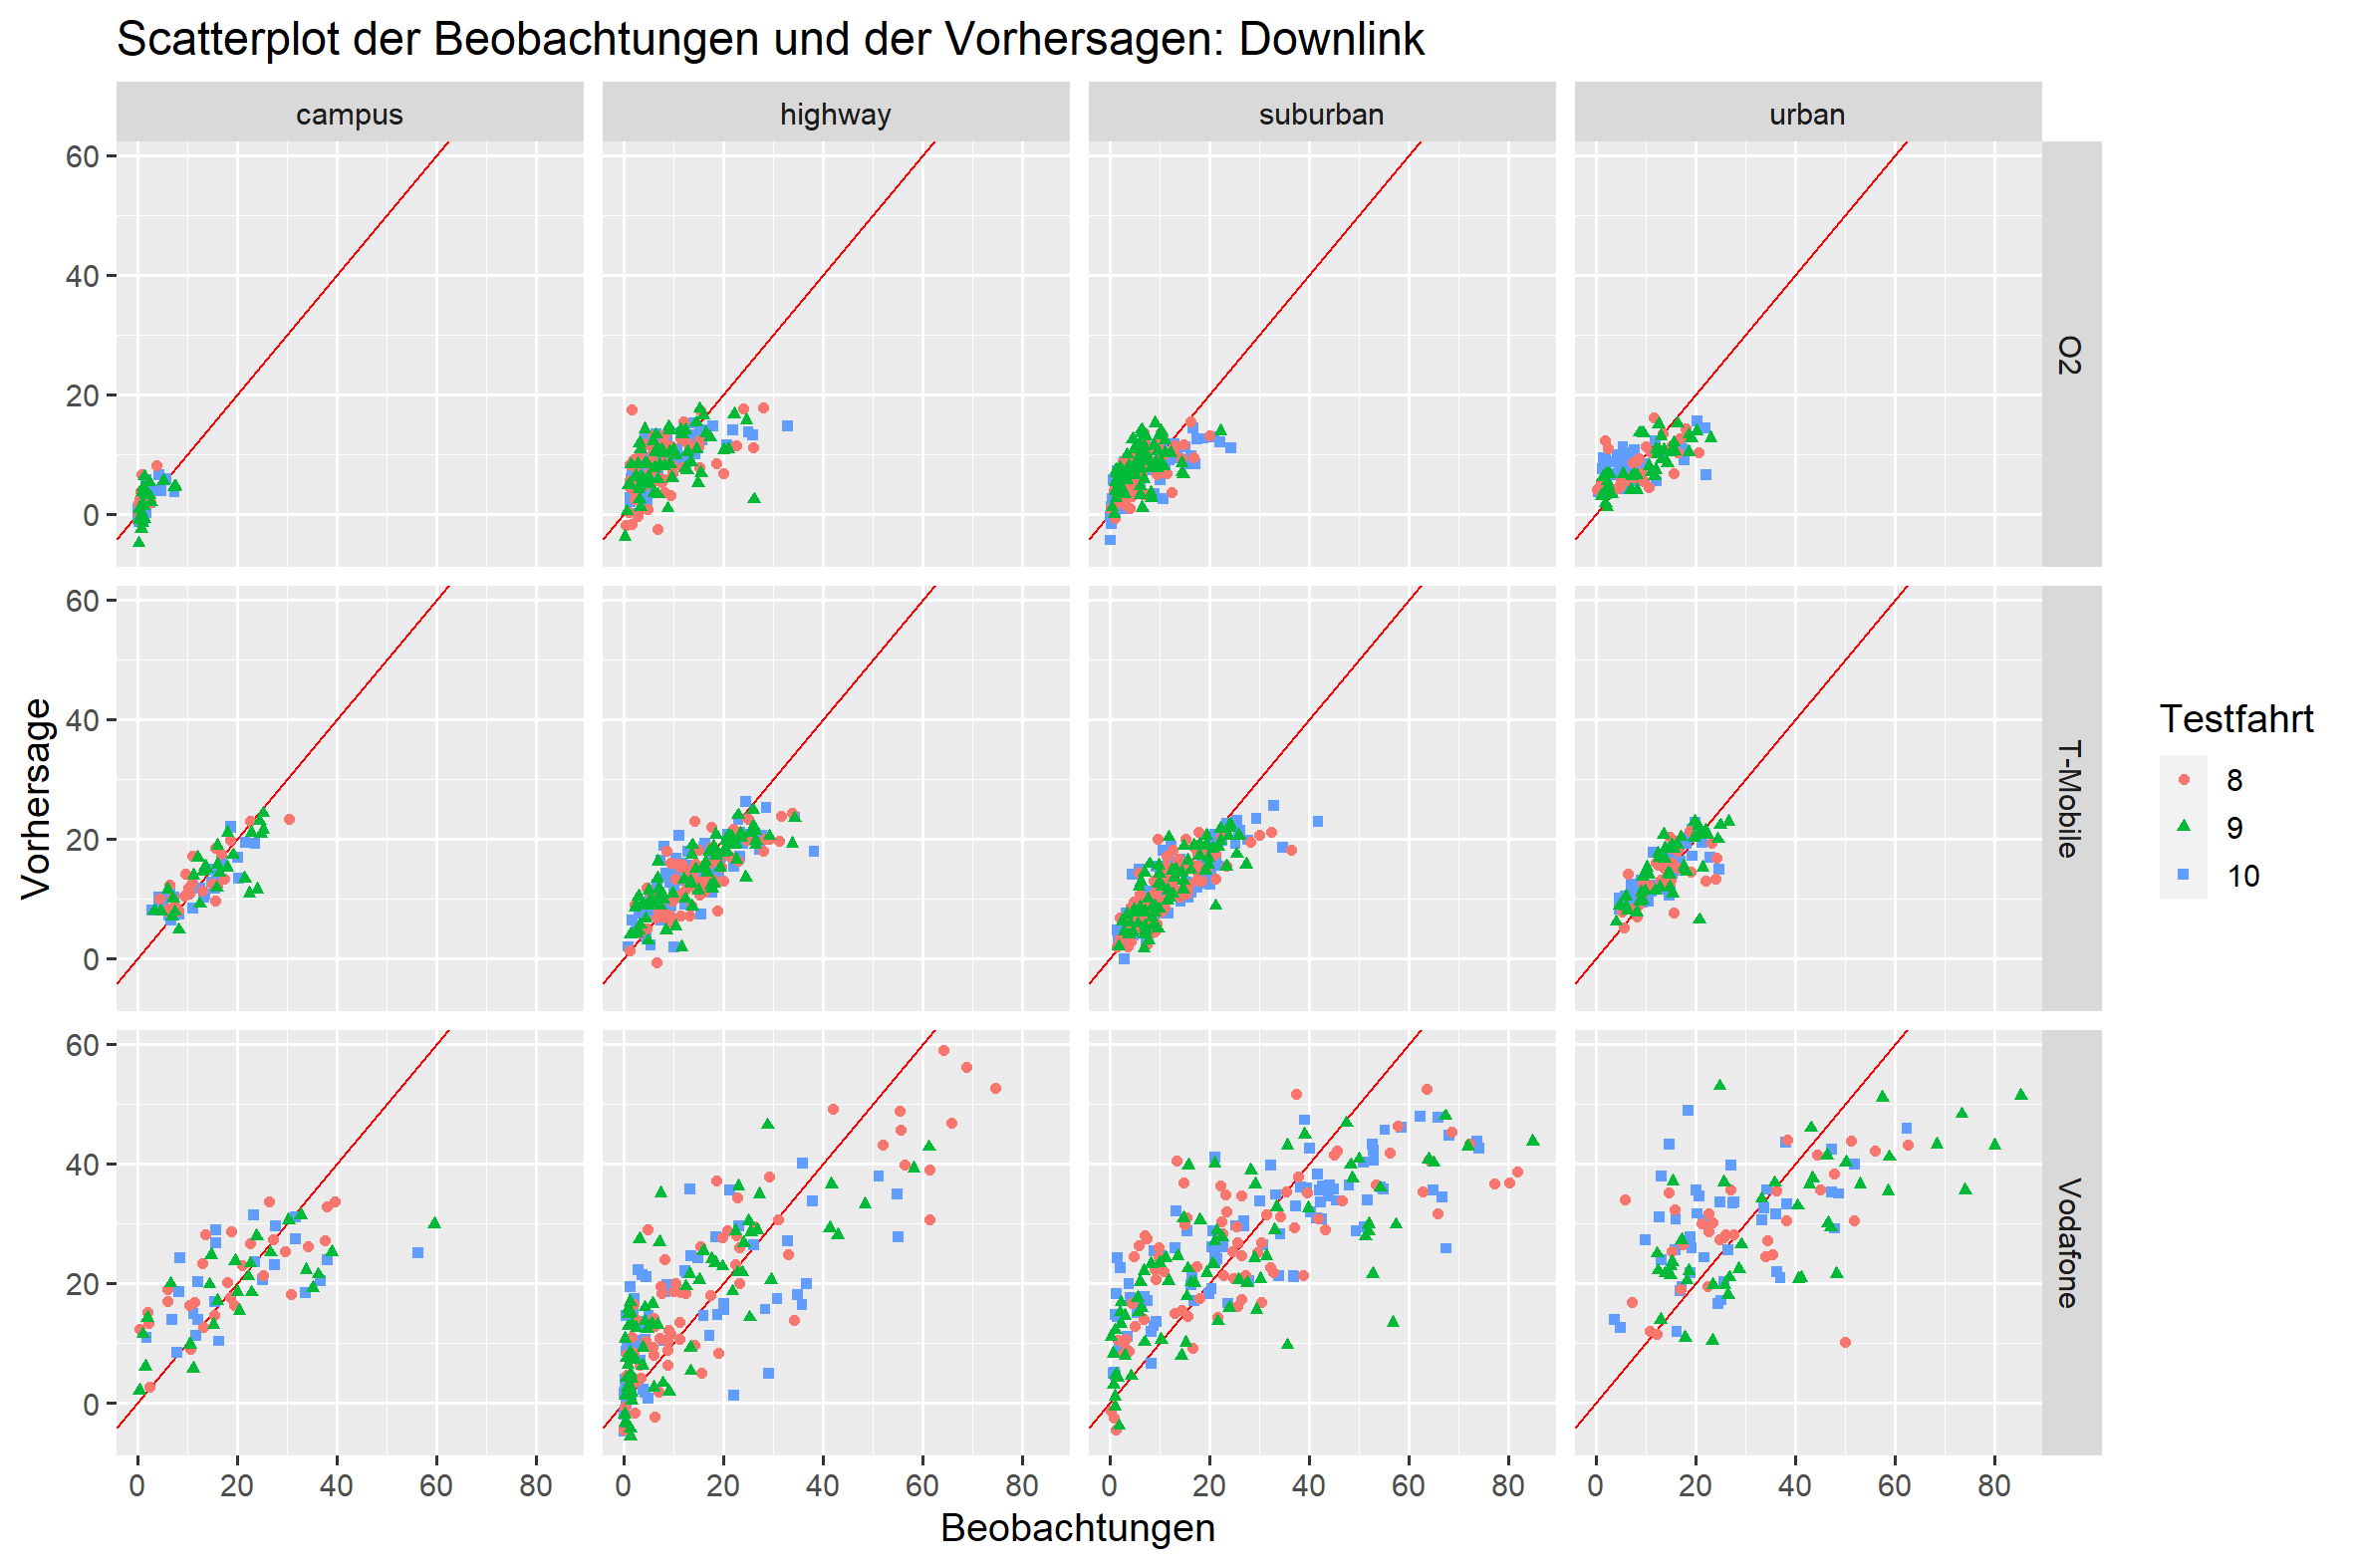
\includegraphics[width=\textwidth]{abbildungen/arma_predictions_dl}
\end{subfigure}
\caption{Out-of-Sample Vorhersagen der Datenraten f\"ur die Regression mit ARMA-Fehlern.}
\label{fig:datarate-predictions-arma}
\end{figure}

\subsubsection{Modellvergleich}

Die betrachteten Kennzahlen $R^2$ und $MAE$ wurden in Abbildung~\ref{fig:kennzahlen-datarate} einander gegen\"ubergestellt.
Man erkennt sofort, dass Extreme Gradient Boosting f\"ur jeden Anbieter die besseren Werte liefert, als die lineare Regression mit
ARMA-Fehlern.
Dies w\"urde die Vermutung best\"atigen, dass das Modell der ARMA-Regression nicht in der Lage ist, s\"amtliche Zusammenh\"ange
in den Daten zu erfassen und das somit das Extreme Gradient Boosting besser zur Vorhersage der Daten\"ubertragungsraten geeignet ist.
\begin{figure}
\centering
\begin{subfigure}{0.49\textwidth}
    \centering
    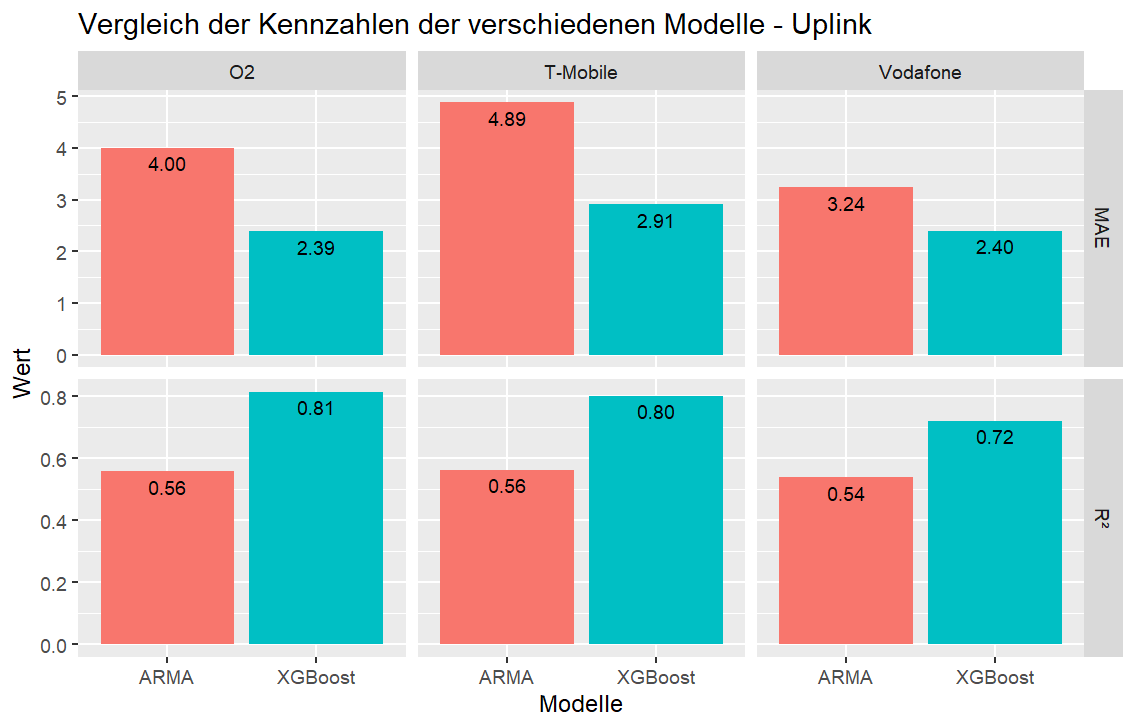
\includegraphics[width=\textwidth]{abbildungen/kennzahlen_vergleich_uplink}
\end{subfigure}
\begin{subfigure}{0.49\textwidth}
    \centering
    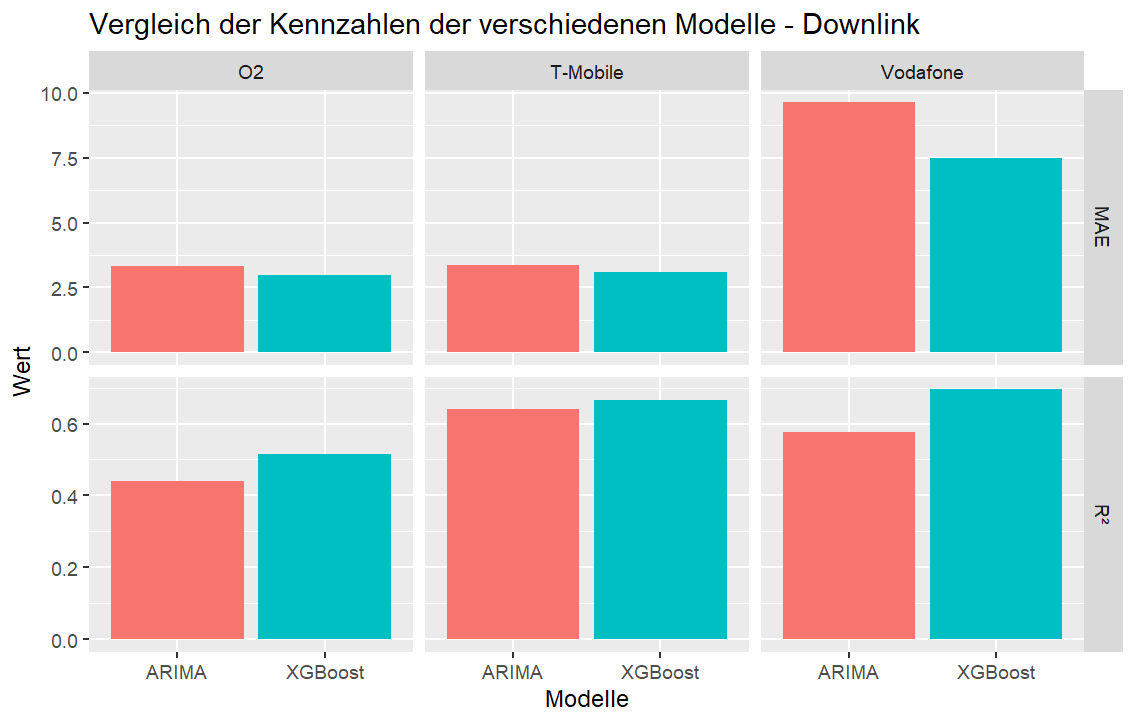
\includegraphics[width=\textwidth]{abbildungen/kennzahlen_vergleich_downlink}
\end{subfigure}
\caption{Vergleich der Kennzahlen f\"ur die Pr\"adiktion der Upload- und Download-Raten.}
\label{fig:kennzahlen-datarate}
\end{figure}

Die Relevanz der einzelnen Kovariablen f\"ur die beiden Pr\"adiktionsmodelle wurde in Abbildung~\ref{fig:feature-importance-datenraten}
dargestellt.
Diese wurden bei der linearen Regression mit ARMA-Fehlern durch die normierte absolute Gr\"o{\ss}e der Modellkoeffizienten ermittelt.
Beim Extreme Gradient Boosting kam die Permutationsmethode zum Einsatz, die Ergebnisse daraus wurden zur besseren Vergleichbarkeit
ebenfalls normiert.

Hierbei f\"allt auf, dass der Variable \textit{Payload} in jeder Situation eine hohe Relevanz besitzt.
F\"ur Exterme Gradient Boosting wird dies sogar besonders deutlich, hier erh\"alt \textit{Payload} in jeder Situation den h\"ochsten
Wichtigkeitswert.
\begin{figure}
\centering
\begin{subfigure}{\textwidth}
    \centering
    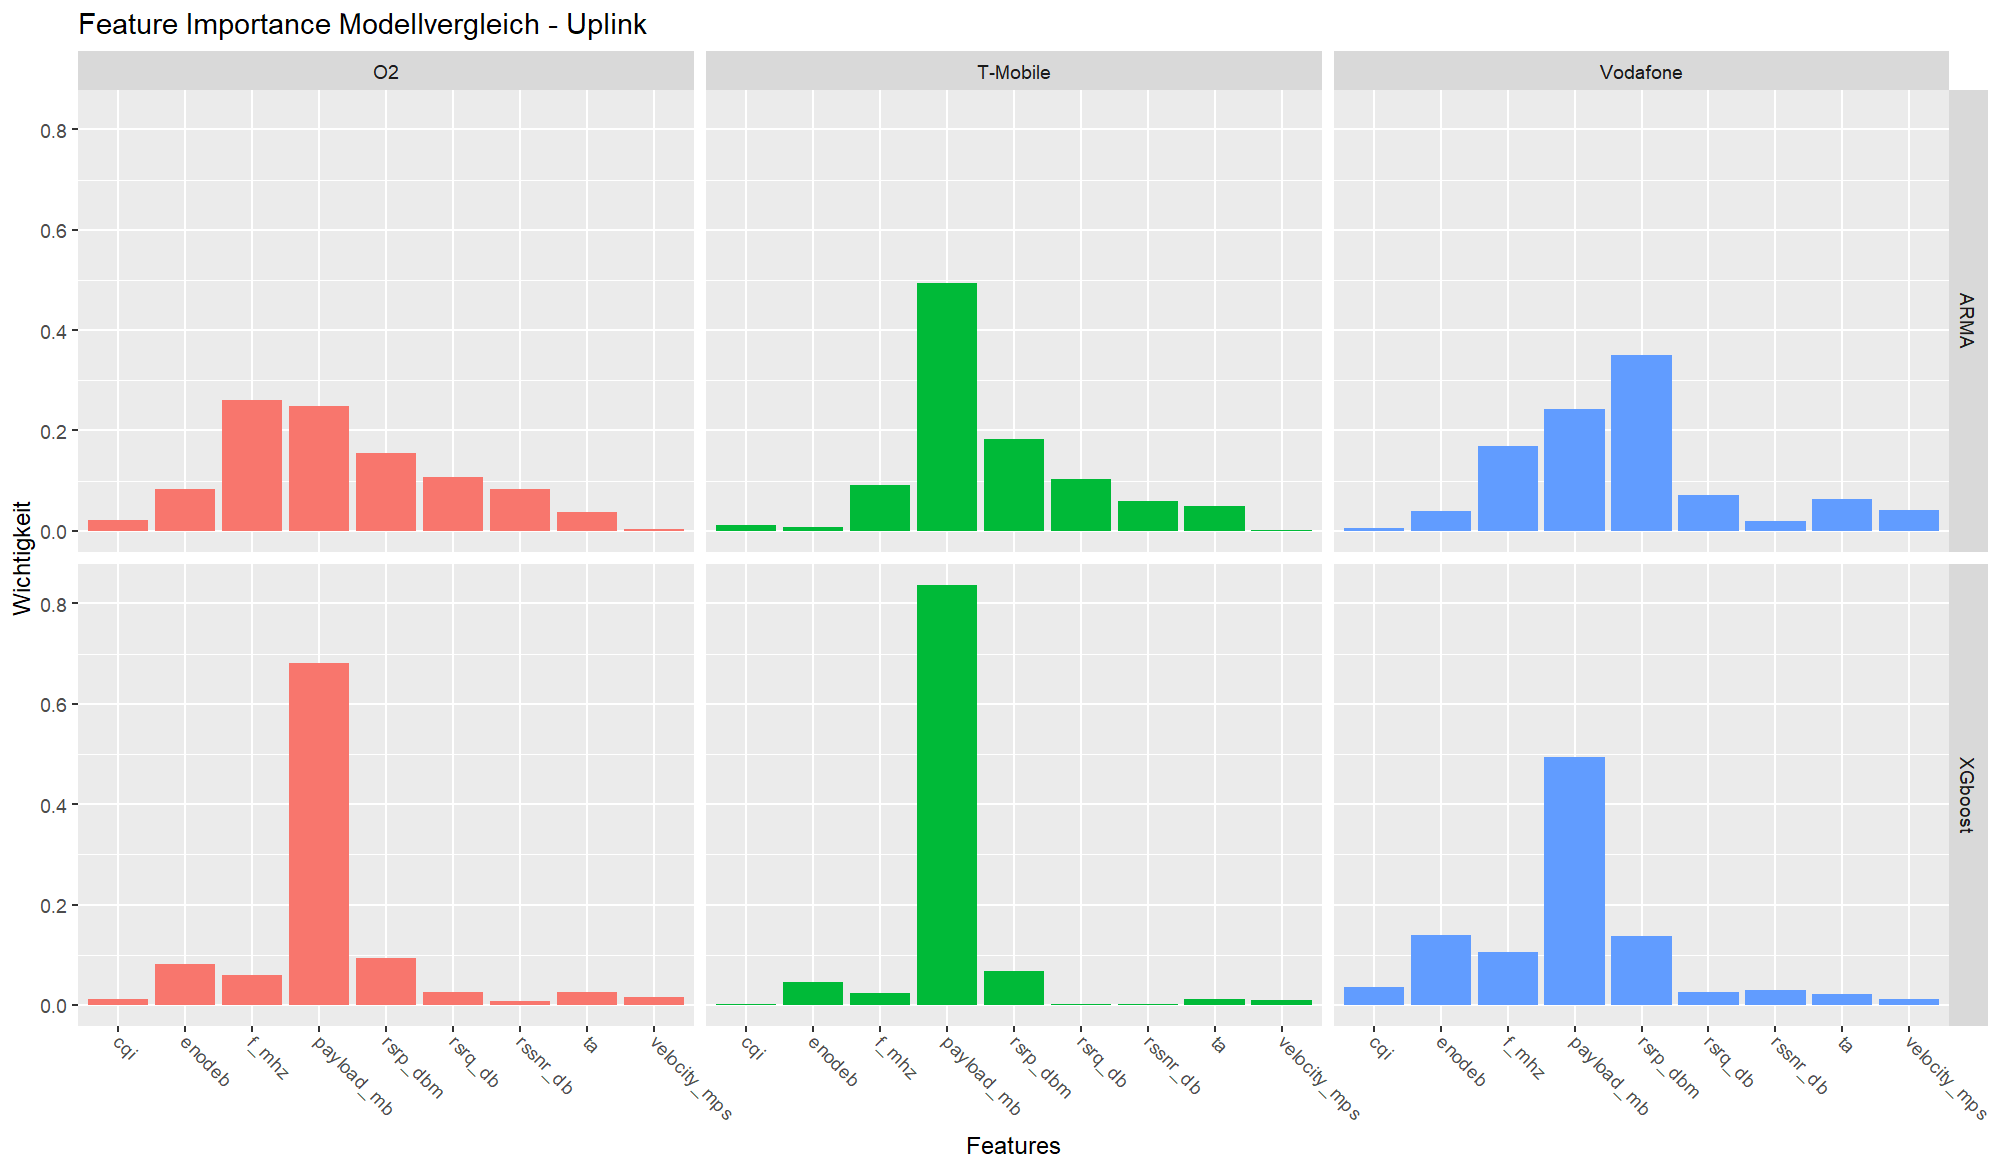
\includegraphics[width=\textwidth]{abbildungen/feature_importance_modellvergleich_uplink}
\end{subfigure}
\begin{subfigure}{\textwidth}
    \centering
    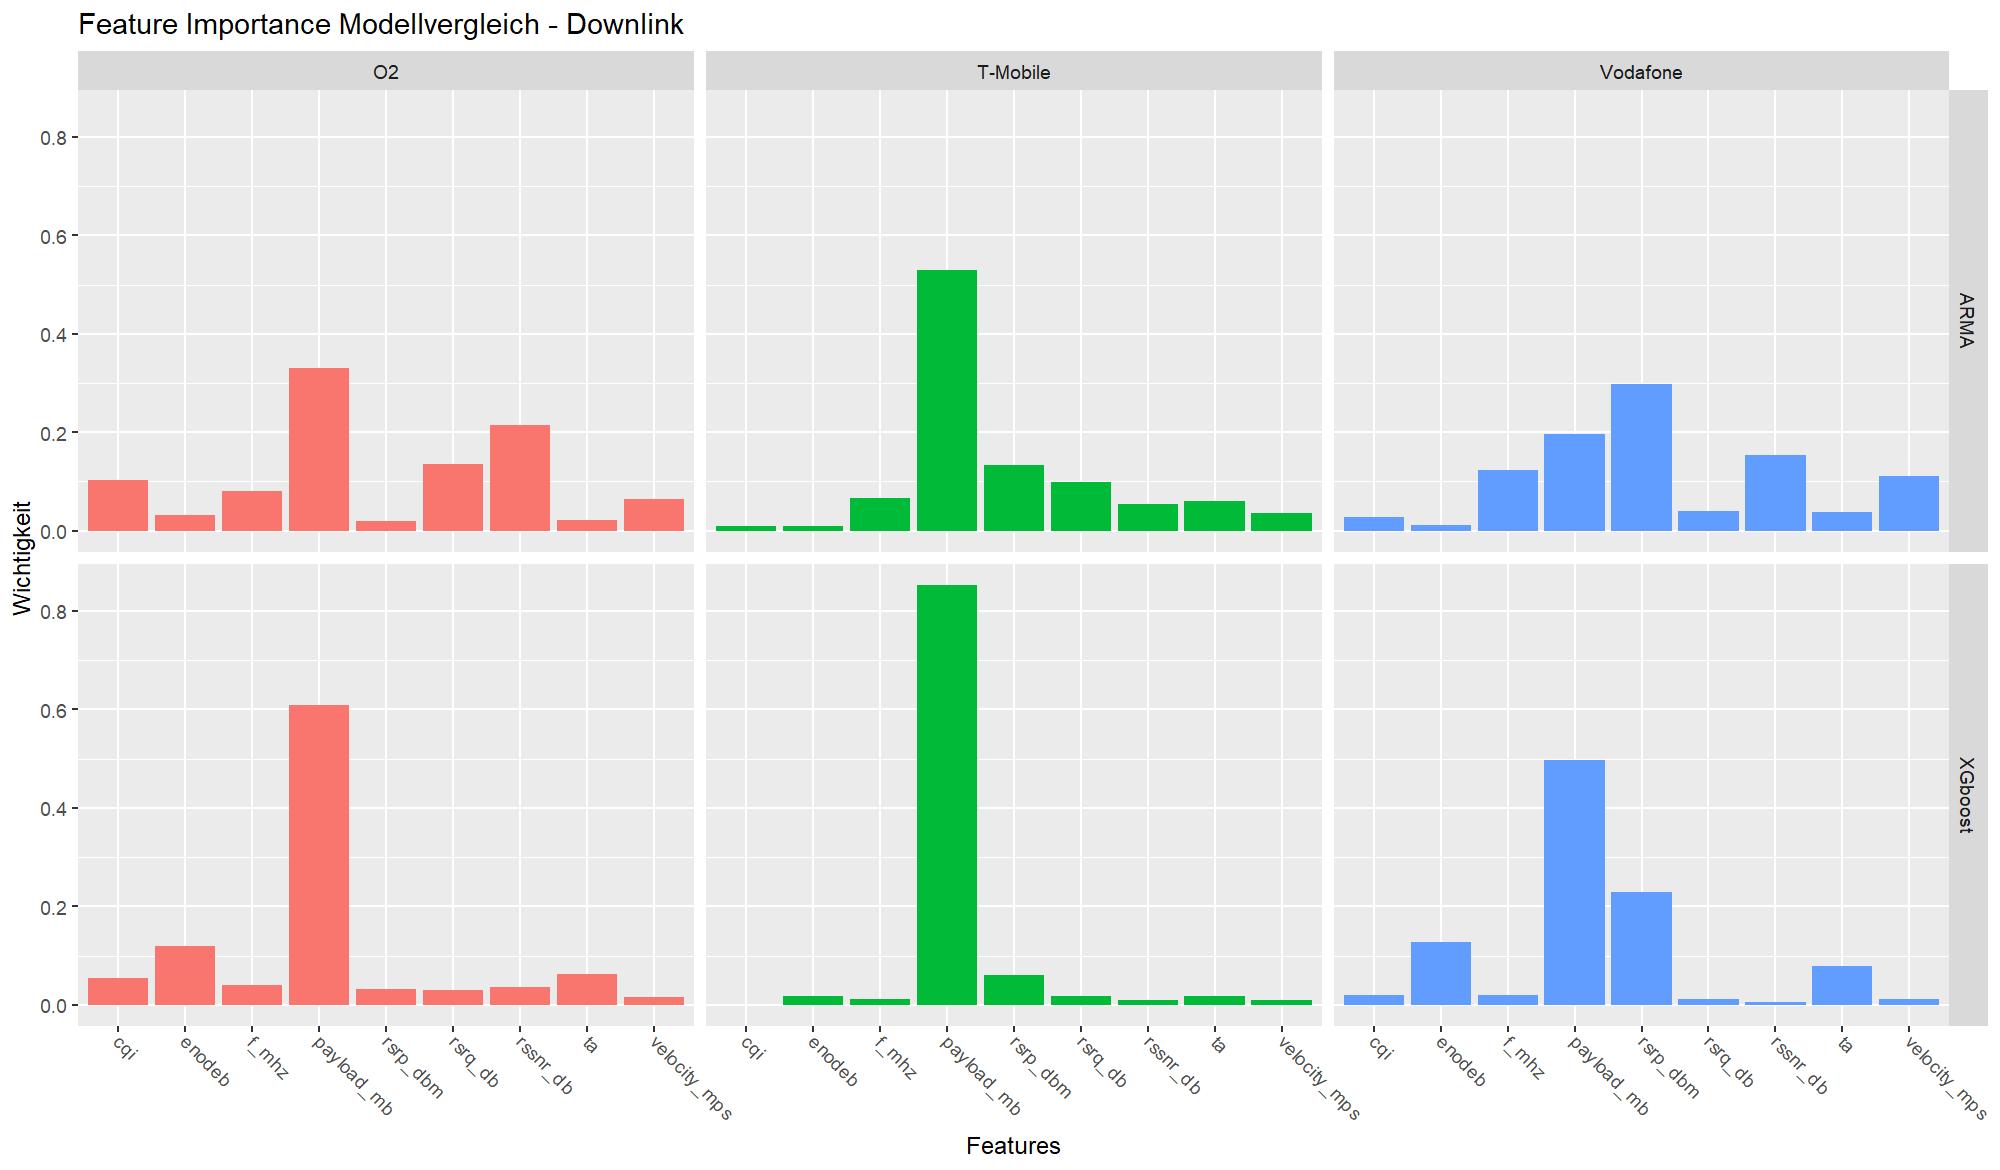
\includegraphics[width=\textwidth]{abbildungen/feature_importance_modellvergleich_downlink}
\end{subfigure}
\caption{Relevanz der Kovariablen bez\"uglich der beiden Modelle zur Datenratenpr\"adiktion.}
\label{fig:feature-importance-datenraten}
\end{figure}

\subsection{Vorhersage der eNodeB-Verbindungsdauern}

Zur Vorhersage der eNodeB-Verbindungsdauern wurde ausschlie{\ss}lich das Extreme Gradient Boosting Modell
eingesetzt. Die Out-of-Sample Vorhersagen hierzu finden sich in Abbildung~\ref{fig:link-lifetime-predictions}.
\begin{figure}
    \centering
    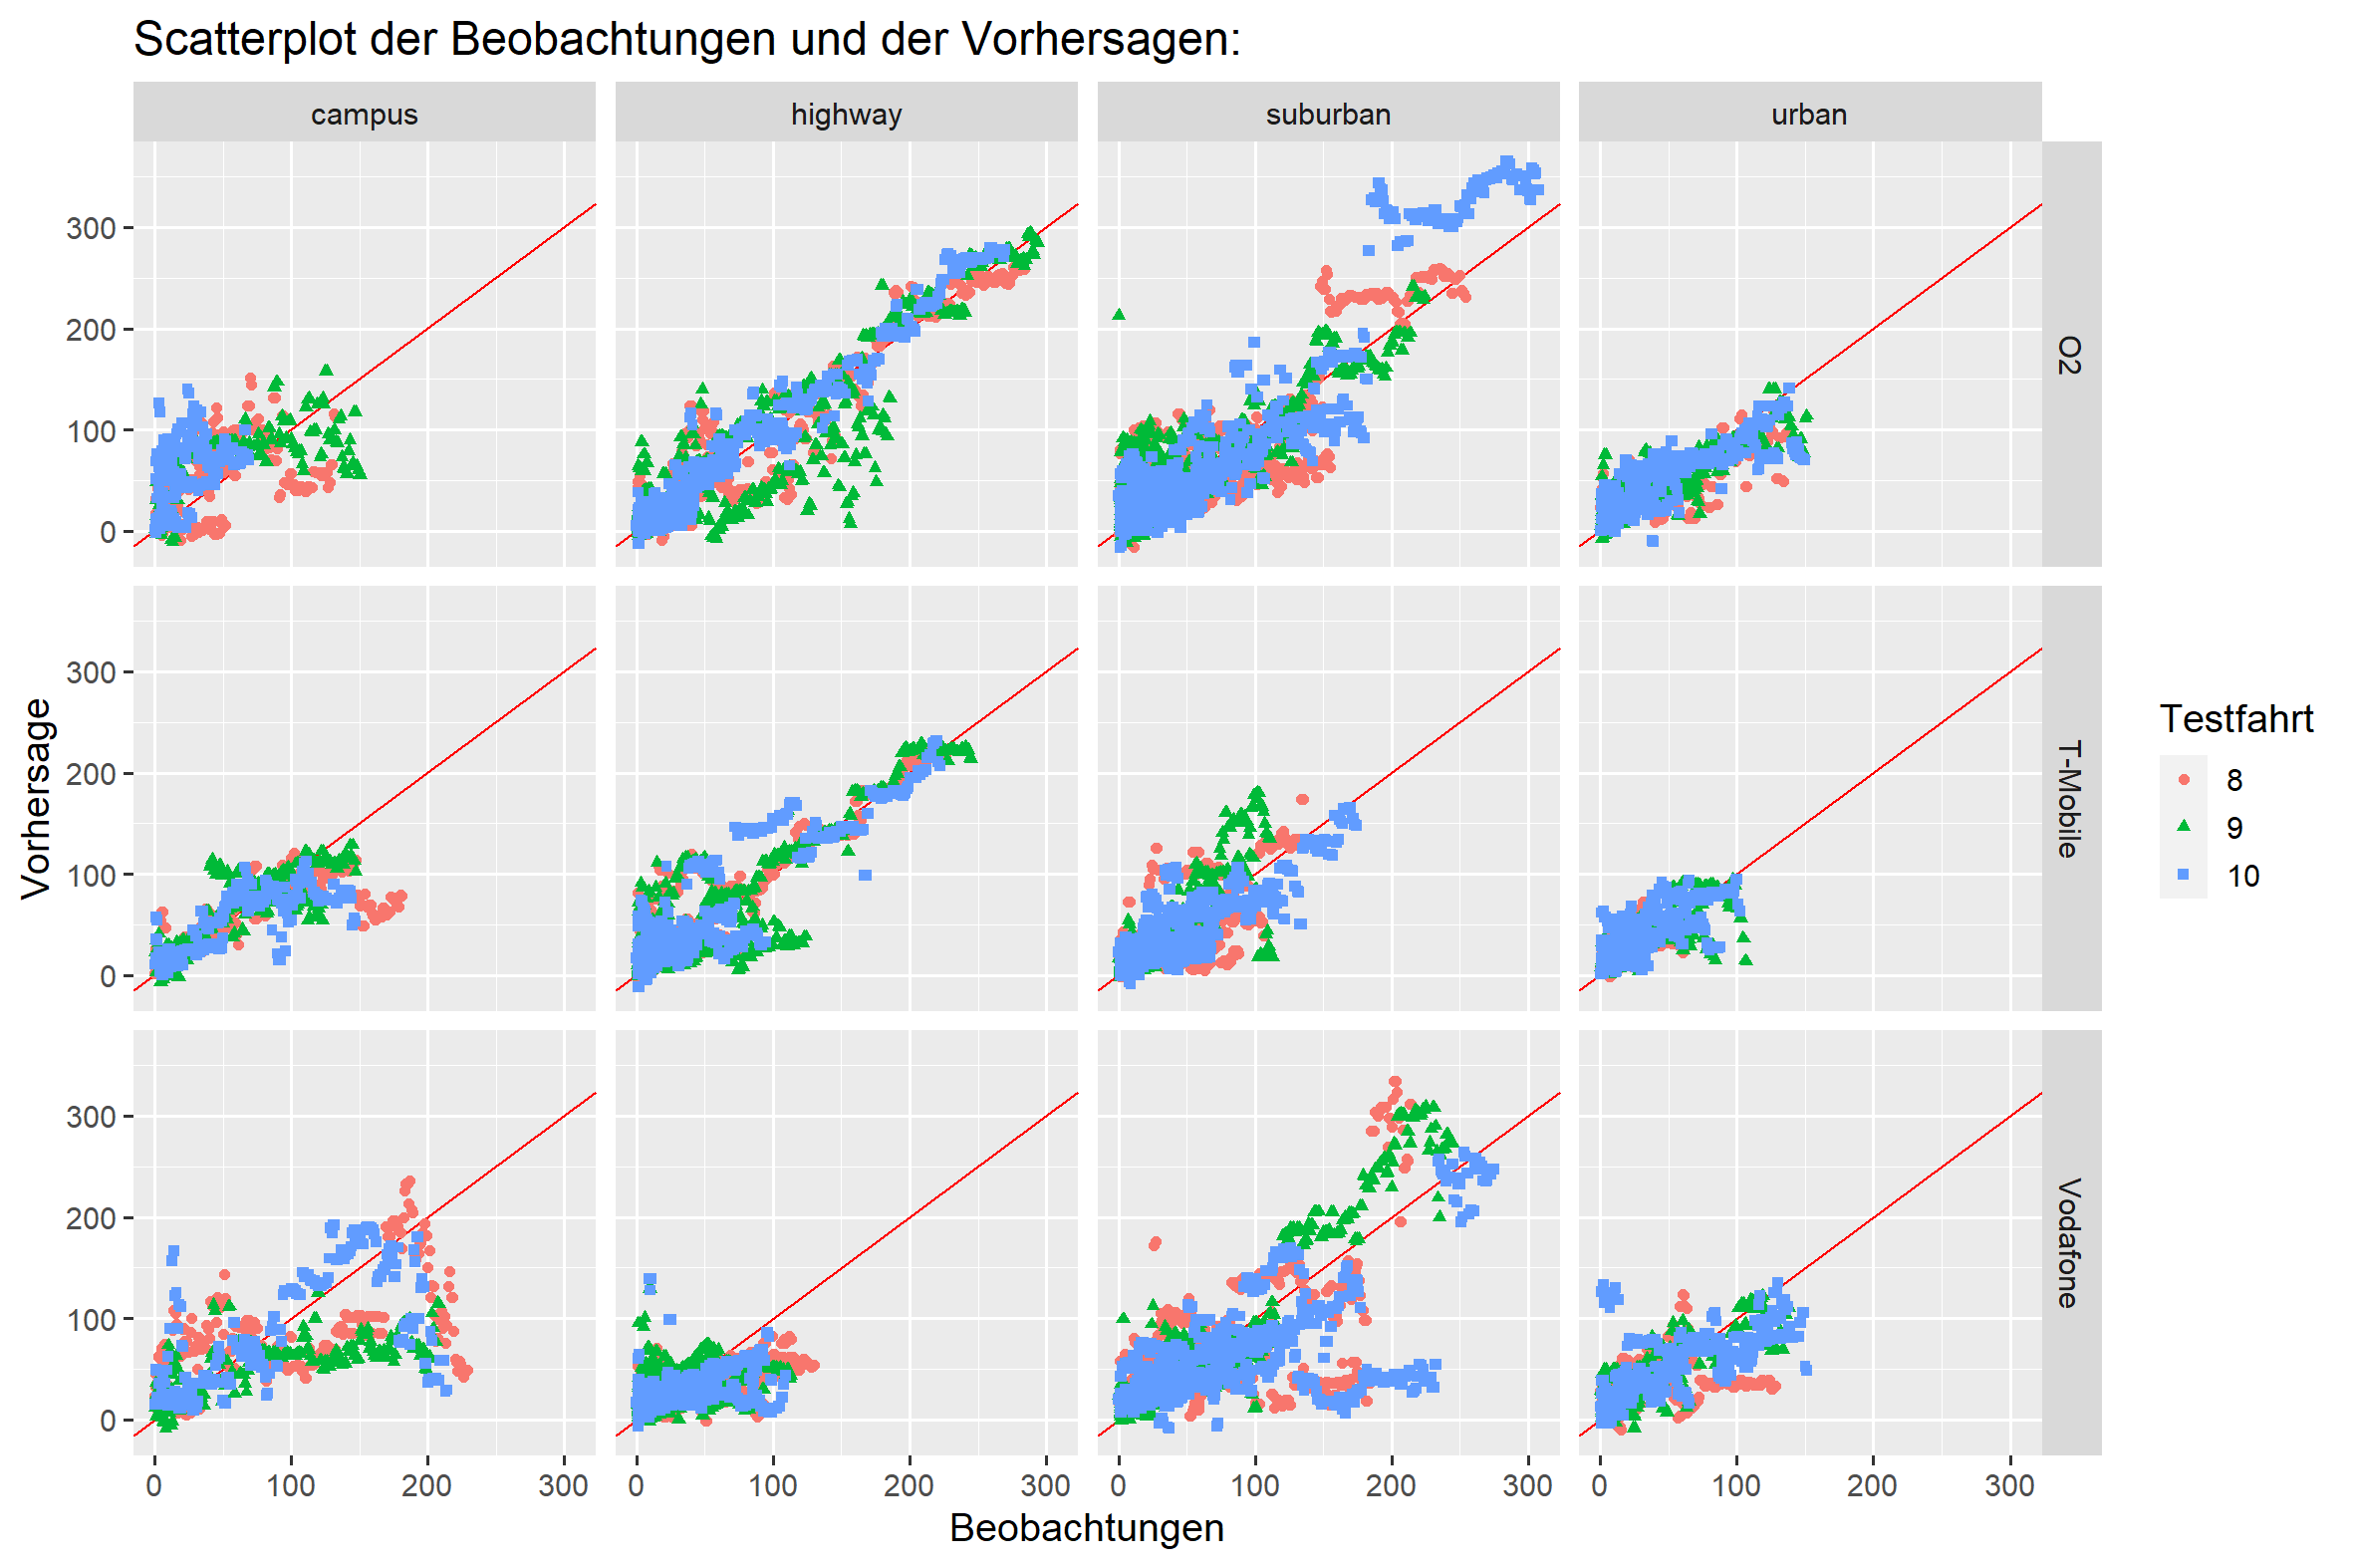
\includegraphics[width=\textwidth]{abbildungen/predictions_linklifetime}
    \caption{Out-of-Sample Vorhersagen der eNodeB-Verbindungsdauern.}
    \label{fig:link-lifetime-predictions}
\end{figure}

\begin{figure}
    \centering
    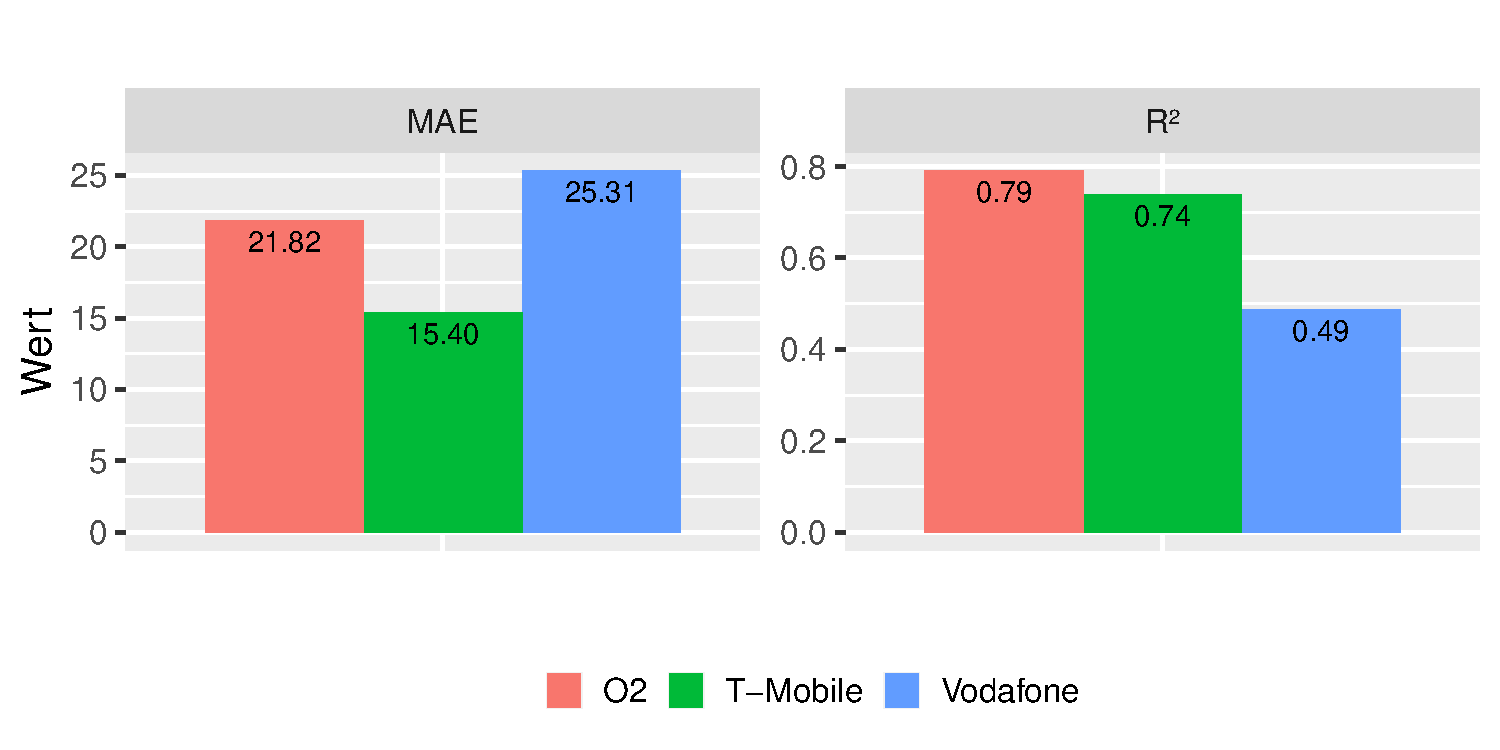
\includegraphics[width=0.5\textwidth]{abbildungen/kennzahlen_linklifetime}
    \caption{Kennzahlen Link-Lifetime.}
    \label{fig:kennzahlen-link-lifetime}
\end{figure}

\begin{figure}
    \centering
    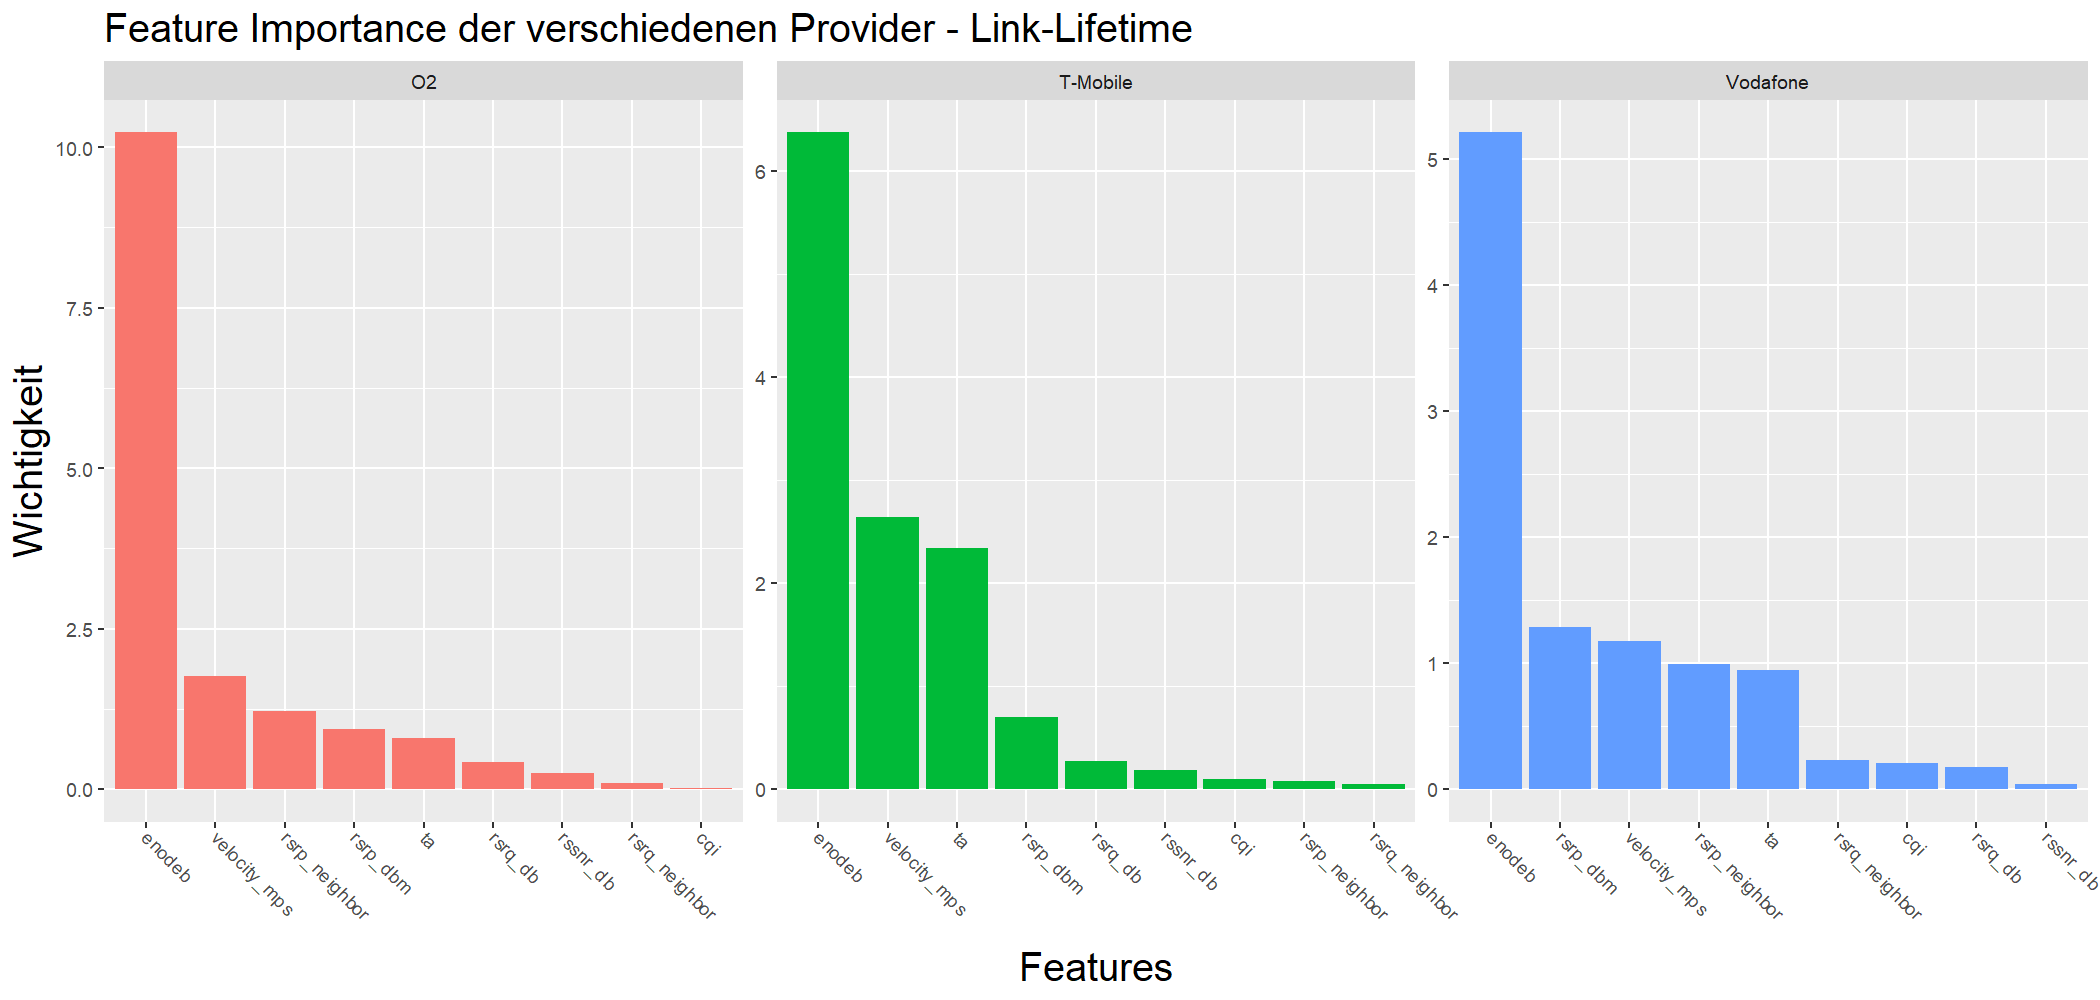
\includegraphics[width=\textwidth]{abbildungen/feature_importance_linklifetime}
    \caption{Feature Importance Link-Lifetime.}
    \label{fig:feature-importance-link-lifetime}
\end{figure}